\chapter{The SpinTaylorF2 waveform model} 

\label{chap:SpinTaylorF2} 
The SpinTaylorF2 waveform~\cite{Lundgren2014} is a single spin, frequency
domain waveform that incorporates the effects of precession.  The waveform
model assumes one component of the binary to have negligible or zero spin, and
describes the inspiral phase of the signal. We will therefore
restrict our attention to NSBH binaries since the neutron star in such
systems are expected to have neglible spins.

\section{Notations and conventions}
Consider a NSBH binary, with black hole mass $m_{1}$ and dimensionless spin
$\chi_{1} = |\mathbf{S}|/m_{1}^2$ where $|\mathbf{S}|$ is the spin angular
momentum of the black hole, and a neutron star with mass $m_{2}$ and zero
spin. The the symmetric mass ratio $\eta$ is defined as $\eta=m_{1}m_{2}/M^2$,
where $M$ corresponds to the total mass of the binary $(m_{1} + m_{2})$.
Further, we can define the total angular momentum vector
$\mathbf{J}=\mathbf{L} + \mathbf{S}$ of the binary as the sum of the orbital
anuglar momentum vector $\mathbf{L}$. We also define the spin-alignment parameter
$\kappa=\hat{\mathbf{L}}\cdot\hat{\mathbf{S}}$, to describe the alignment of
the $\mathbf{L}$ and $\mathbf{S}$: $\kappa=0$ corresponds to the situation
where $\mathbf{L}$ and $\mathbf{S}$ are perpendicular to each other, and
$\kappa=\pm 1$ correponds to the aligned (anti-aligned) case. In addition,
polar angles $(\theta_{J}, \psi_{J})$  describes the relative orientation  of
the total angular momentum vector $\mathbf{J}$ with the line of sight unit
vector $\hat{\mathbf{N}}$ (see, for eg.,~\cite{thetaJ} for a graphical
representation of the coordinates used). All the equations in the report are
written in $\left[G = c = M_{\odot }= 1\right]$ units.

\section{Inertial and co-rotating frames of reference}

\label{fig:frames} 
\begin{figure}[t]
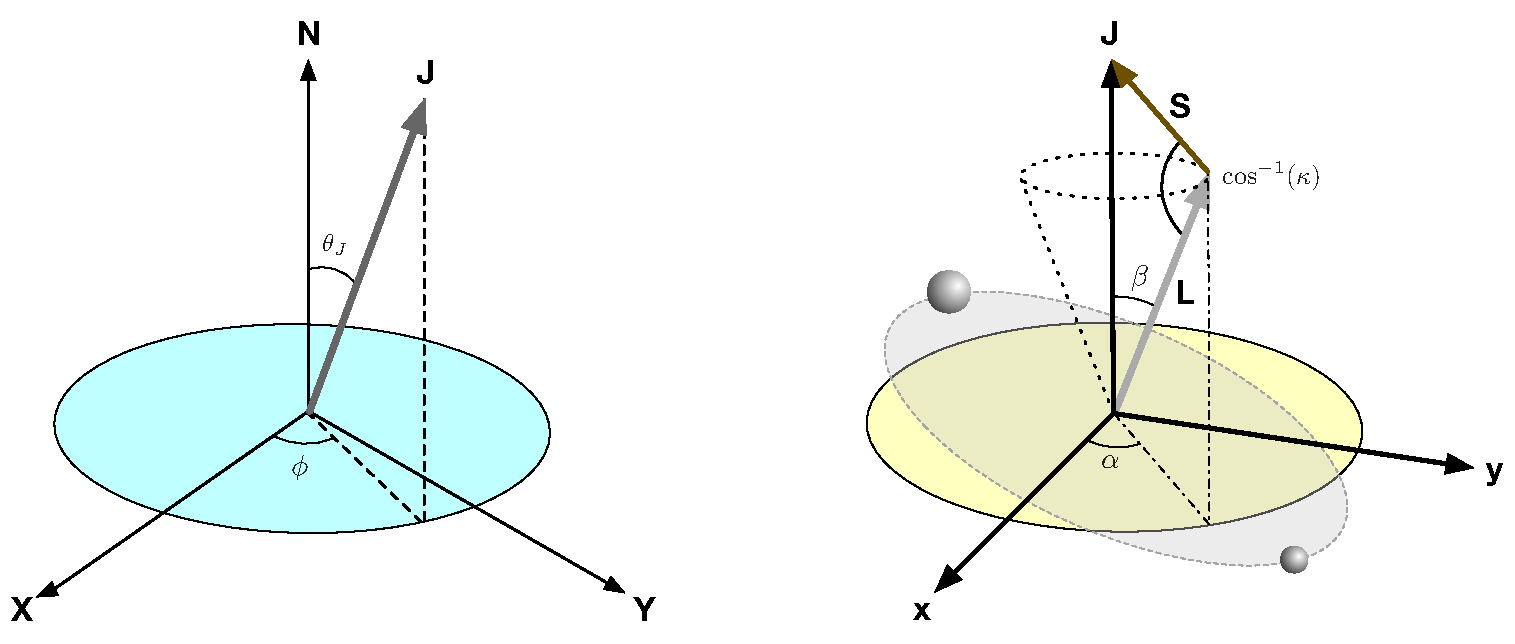
\includegraphics[width=\textwidth]{./images/STF2_coordinates.pdf}
\caption{Detector (left) and inertial frame (right) of reference for
precessing systems.}
\centering 
\end{figure}

If the black hole has non-zero spin, and the spin-angular momentum
$\mathbf{S}$ is  not aligned with the orbital orbital angular momentum
$\mathbf{L}$ of the binary, the plane of orbital motion inclines and precesses
over time~\cite{Apostolatos1994}. Concretely, both $\mathbf{L}$ and
$\mathbf{S}$  would precess about the total angular momentum vector
$\mathbf{J}$ (see Eq.~(11) in~\cite{Apostolatos1994} for evolution equations
of $\mathbf{L}$ and $\mathbf{S}$). Further, if $\mathbf{L}$ and $\mathbf{S}$
do not cancel each other (i.e. are not antialigned and almost equal in
magnitude)  the binary undergoes simple precession\footnote{The SpinTaylorF2
waveform assumes simple precession~\cite{Lundgren2014}, and breaks down  when
the assumption is no longer applicable.}~\cite{Apostolatos1994}, where
$\mathbf{J}$ remains nearly fixed during the inspiral, and $\mathbf{L}$ and
$\mathbf{S}$ precesses about $\mathbf{J}$ with a uniform angular velocity.

To describe the dynamics of the system, therefore, we introduce two different
frames of reference. The first frame (called the inertial or observer's frame
of reference) is aligned with the total angular momentum vector $\mathbf{J}$,
and, therefore fixed in space. The other frame co-rotates with the orbital
plane, i.e., is always instantaneouly aligned with the direction of the
orbital angular momentum, and is therefore referred to as the non-inertial
(co-rotating) frame of reference. See Fig.~\ref{fig:frames}, which shows the
orientation of $\mathbf{J}$ and $\mathbf{L}$ with the detector frame (left)
and inertial frame (right), respectively. 

Note that the inertial frame is not the same detector frame (though both of
them are fixed in space) but is related to it by a rotation via the angles
$(\theta_J,\psi_J)$, whereas the inertial frame and the co-rotating frame are
related to each other by a time- dependent rotation expressed in terms of the
Euler angles $(\alpha, \beta,
\gamma)$.

\label{fig:waveforms} 
\begin{figure}[t]
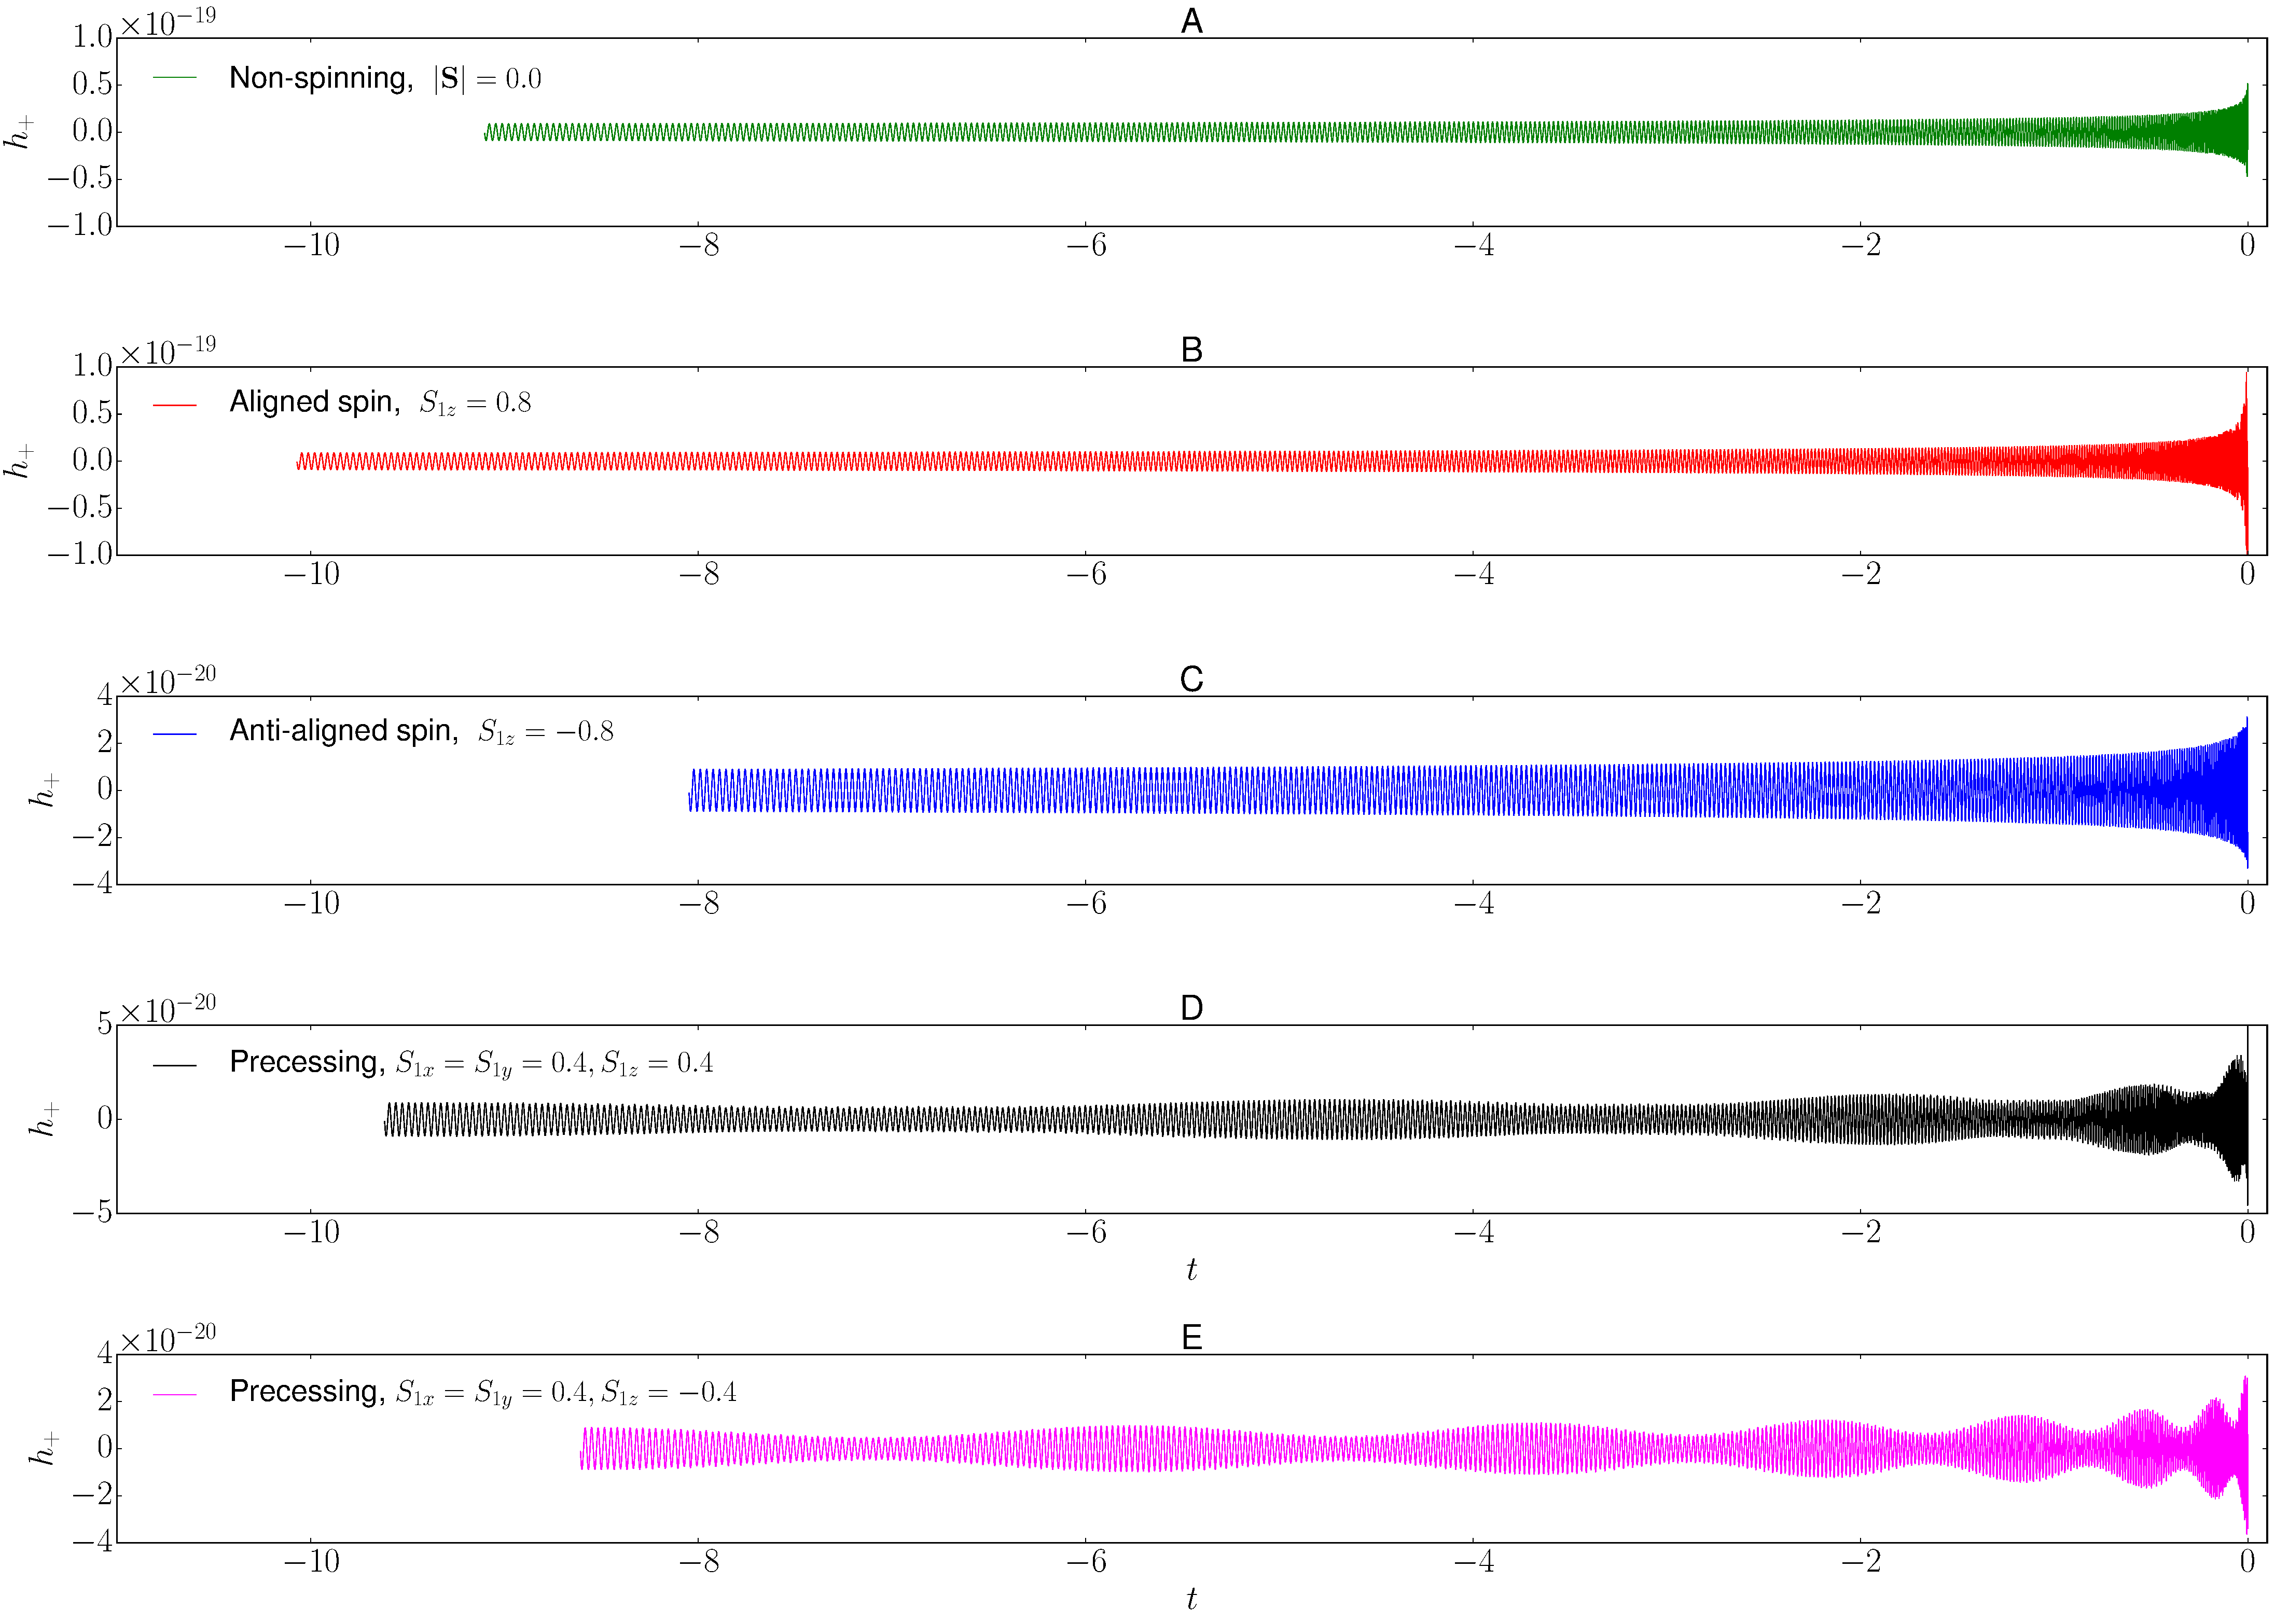
\includegraphics[width=\textwidth]{./images/SPT2_waveforms.pdf}
\caption{SpinTaylorT2 waveforms for non-precessing (A, B, C) and precessing
(D, E) systems.}
\centering 
\end{figure}

\section{The construction of SpinTaylorF2}

The precession of the orbital plane leads to modulations in the gravitational
wave amplitude and phase in the observer's frame of reference (see
Fig.~\ref{fig:waveforms}). The waveforms are modulated both in amplitude and
phase, because of the precession of $\mathbf{L}$ and $\mathbf{S}_1$ about
$\mathbf{J}$. From the figure, the effect of precession on waveform amplitude
is evident. In addition to the inspiral time scale, the precession introduces
a new time scale which is responsible for the waveform modulation. Further,
the rate of precession also changes during the inspiral phase (depending on
the spin alignment parameter $\kappa$), which in turn introduces
characteristic variations in the modulations of the waveform. For example,
$\kappa < 0$ introduces more modulations, and therefore stronger precession,
compared $\kappa > 0$; compare panels (D) and (E).


Schmidt et al. showed that precessing waveform in the inertial frame of
reference can be \textit{approximately mapped} into a non-precessing waveform acted
upon by a time-dependent rotation~\cite{Schmidt2012}, which was further
refined by~\cite{Boyle2011, Rotation}. The time-dependent rotation relates the
inertial frame of reference aligned with $\mathbf{J}$ to a frame that co-rotates 
with the precession of the orbital angular momentum vector
$\mathbf{L}$. The precessing waveform can then be expressed as a weighted sum
of the co-rotating frame amplitudes $\tilde{h}^{l,m}$ (see Eq. (3)
in~\cite{Lundgren2014}):
\begin{equation}   
h_{+} + i h_{\times} = e^{-2 \psi}
\sum_{l,m,m^{\prime}} \mathcal{D}^{l}_{m^{\prime},m} \left(\alpha, \beta, \gamma\right)
\tilde{h}^{l,m}(t){}_{-2}Y_{l,m^{\prime}}\left(\theta,\phi\right)e^{-i m \Phi},
\end{equation}   
where $\mathcal{D}^{l}_{m^{\prime},m}$ is the Wigner rotation matrix of
SU2~\cite{Boyle2011}, and $(\alpha, \beta, \gamma)$ are the time-dependent
Euler angles that relate the co-rotating frame to the inertial frame of
reference, and $\Phi$ is orbital phase of the waveform.
See~\cite{Lundgren2014} for complete definitions. Considering only the leading
order $(l=2, |m| = 2)$ mode, we can express the above expression in frequency
domain using the stationary phase approximation~\cite{Lundgren2014,
Creighton}.  Upon simplification, one arrives at the following expression for
the SpinTaylorF2 waveform (see Eq. (12--13) in~\cite{Lundgren2014}):
\begin{equation}  
\label{STF2_main} 
h_{+}(f) =
\dfrac{2\pi M_{c}^{2}}{D}\sqrt{\dfrac{5}{96\pi}}(\pi M
f)^{-7/6}\sum_{m}z_{m}e^{i(\Psi - 2\zeta) + i m \alpha},
\end{equation} 
where $D$ corresponds to the distance to the source, and $M_{c}$ corresponds to
chirp mass~\cite{Creighton} of the binary. The expressions for $\alpha,
\Psi$ and $\zeta$  can be found in~\cite{Lundgren2014}, we omit them for
brevity. Each term in the summation in Eq.~(\ref{STF2_main}) represents a
single sideband that is modulated in amplitude and phase depending on the
value of $m$. We observed that in  the non-precessing case, only the $m=2$
sideband has a non-zero amplitude; however, for a precessing system, all the
sidebands develop a non- zero amplitude. Thus, we would expect that the single
to noise ratio (SNR) from the total waveform would be sub-divided into the SNR
contribution from each of the individual sidebands in case of precession
systems. In the following chapter, we discuss how the SNR of the total
waveform is distributed among the sidebands by computing overlap between the
particular sideband and the full waveform.






